\documentclass{article}
\usepackage{amsmath}
\usepackage{graphicx}
\usepackage{listings}

\begin{document}

\section*{PROBLEM STATEMENT}
To implement 2D rotation transformation using OpenGL in C and to draw and rotate a polygon against a defined coordinate system. The program will also draw the coordinate axes for better visualization.

\section*{THEORY}
2D rotation is a geometric transformation that rotates an object about the origin (0, 0) in a 2D plane by a specified angle \(\theta\). The rotation transformation is described by the rotation matrix:

\[
R(\theta) = \begin{bmatrix}
\cos\theta & -\sin\theta \\
\sin\theta & \cos\theta
\end{bmatrix}
\]

When a point \((x, y)\) is rotated, the new coordinates \((x', y')\) are computed as:
\[
x' = x \cos\theta - y \sin\theta
\]
\[
y' = x \sin\theta + y \cos\theta
\]

\section*{ALGORITHM}

\begin{enumerate}
    \item Initialize the coordinates of the polygon vertices.
    \item Draw the coordinate axes using the Bresenham line drawing algorithm.
    \item Draw the original polygon.
    \item Apply the rotation transformation to each vertex of the polygon.
    \item Draw the rotated polygon in a different color.
\end{enumerate}

\section*{FLOWCHART}
\begin{center}
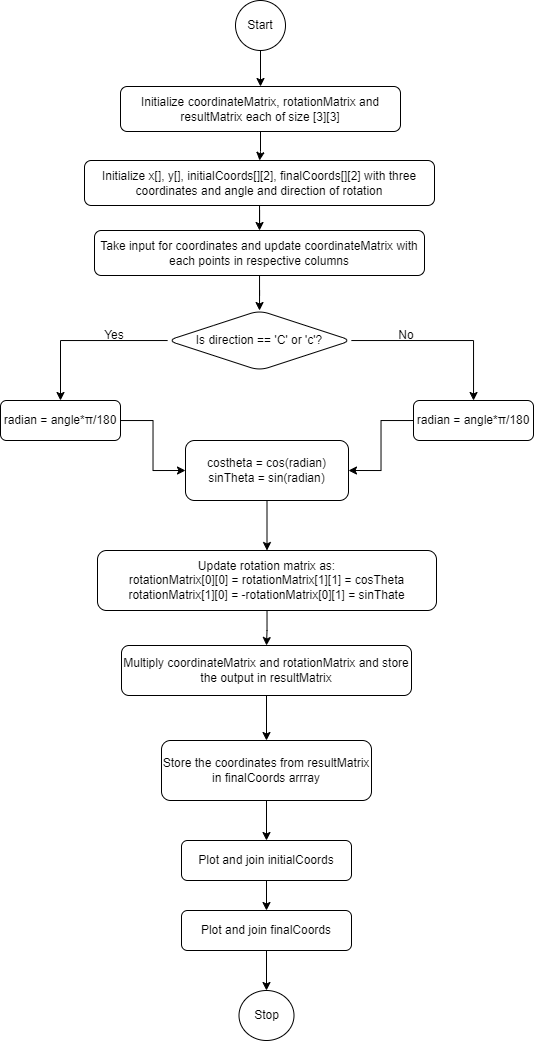
\includegraphics[width=0.7\textwidth]{flowchart.png}
\end{center}

\section*{SAMPLE I/O}
\textbf{Input:}
\begin{verbatim}
Polygon vertices: (10, 10), (200, 10), (200, 200), (10, 200)
Rotation angle: 45 degrees
\end{verbatim}

\textbf{Output:}
The original and rotated polygons are displayed in a window with coordinate axes.

\section*{DISCUSSIONS}
\begin{itemize}
    \item \textbf{Advantages}: Rotation is a fundamental transformation in graphics, allowing for the orientation change of objects. It is mathematically simple to implement.
    \item \textbf{Disadvantages}: Rotation about points other than the origin requires additional transformations, which can complicate the implementation.
    \item \textbf{Applications}: Rotation is widely used in graphics, animation, CAD software, and game development for changing the orientation of objects and models.
\end{itemize}

\section*{CONCLUSION}
The 2D rotation transformation is essential in computer graphics for changing the orientation of objects. Implementing this transformation using OpenGL provides a visual understanding of how rotation affects the position and orientation of a polygon. Drawing coordinate axes helps in better visualization of the transformation effects.


\end{document}
